\section{Công đoạn chung của phương pháp học sâu trong bài toán sinh cử chỉ}
\label{sec:commonstage}

Như đã trình bày ở \autoref{sec:Data}, cử chỉ bao gồm chuỗi chuyển động của tọa độ điểm 3D. Với mỗi tập dữ liệu số lượng xương (bone) mỗi khung hình sẽ khác nhau. 

Cách tiếp cận bằng học sâu với bài toán sinh cử chỉ (gesture generation) được thực hiện với nhiều phương pháp khác nhau. Tuy nhiên luận văn tổng quát hóa lại thành các công đoạn chính như \autoref{fig:CommonStage} sau:

\begin{figure}[H]
	\centering
	\includegraphics[width=\textwidth]{CommonStage}
	\caption{Các công đoạn trong mô hình sinh cử chỉ.}
	\label{fig:CommonStage}
\end{figure}

\begin{enumerate}[label=\textbf{\arabic*.}]
	\item \textbf{Tiền xử lý dữ liệu} (Preprocessing): Trong công đoạn tiền xử lý, các dữ liệu về đoạn giọng nói, dữ liệu về chuỗi cử chỉ, đoạn văn bản sẽ được đọc, số hóa để thu được các vector hoặc ma trận thể hiện thông tin thô của dữ liệu. Đối với mỗi phương pháp học khác nhau, các thông tin dữ liệu ban đầu sẽ được chọn để học cũng khác nhau.
	
	\item \textbf{Xử lý đặc trưng} (Feature Processing): Trong công đoạn xử lý đặc trưng, các dữ liệu thô như giọng nói và văn bản được nhúng (embedding) để biểu diễn thành các vector đặc trưng. Các phương pháp khác nhau sẽ chọn các mô hình nhúng khác nhau. Việc biểu diễn các cử chỉ của nhân vật thành các vector đặc trưng của mỗi phương pháp cũng khác nhau.
	
	\item \textbf{Trích xuất đặc trưng} (Feature Extraction): Công đoạn trích xuất đặc trưng sẽ dùng các lớp biến đổi tuyến tính (linear) hoặc các lớp CNN để trích xuất các đặc trưng của dữ liệu. Các dữ liệu về văn bản hoặc giọng nói sau khi xử lý đặc trưng có thể cũng được cho đi qua các lớp trích xuất đặc trưng để biểu diễn thành các vector đặc trưng để biểu diễn tương ứng với văn bản và giọng nói.
	
	\item \textbf{Mã hóa đặc trưng} (Feature Encoding): Trong công đoạn mã hóa đặc trưng, các vector về cử chỉ, cảm xúc, và giọng nói sẽ được biểu diễn lên không gian tiềm ẩn nhỏ hơn kích thước ban đầu nhằm thuận tiện cho việc tính sự tương quan giữa các đặc trưng ở công đoạn kết hợp đặc trưng.
	
	\item \textbf{Kết hợp đặc trưng} (Feature Fusion): Trong công đoạn kết hợp đặc trưng, các đặc trưng giọng nói, văn bản, cử chỉ cũng như các thông tin khác được kết hợp với nhau bằng việc concat, các lớp kết nối đầy đủ hoặc kết hợp các đặc trưng bằng cách cộng hoặc trừ các vector tiềm ẩn.
	
	\item \textbf{Giải mã đặc trưng} (Feature Decoding): Trong công đoạn giải mã đặc trưng, các vector tiềm ẩn sẽ được giải mã hay tăng chiều dữ liệu về kích thước ban đầu.
	
	\item \textbf{Kết xuất} (Render): Sau khi có được vector ở kích thước ban đầu, các vector sẽ được biến đổi ngược trở về các tệp BVH để được kết xuất thông qua các phần mềm như Blender hoặc Unity để minh họa các chuyển động nhân vật.
\end{enumerate}

\section{Diffusion-base Model}
\label{sec:diffusionbase}

\subsection{Nguyên lý chung của các phương pháp dựa trên Diffusion}

\begin{figure}[H]
	\centering
	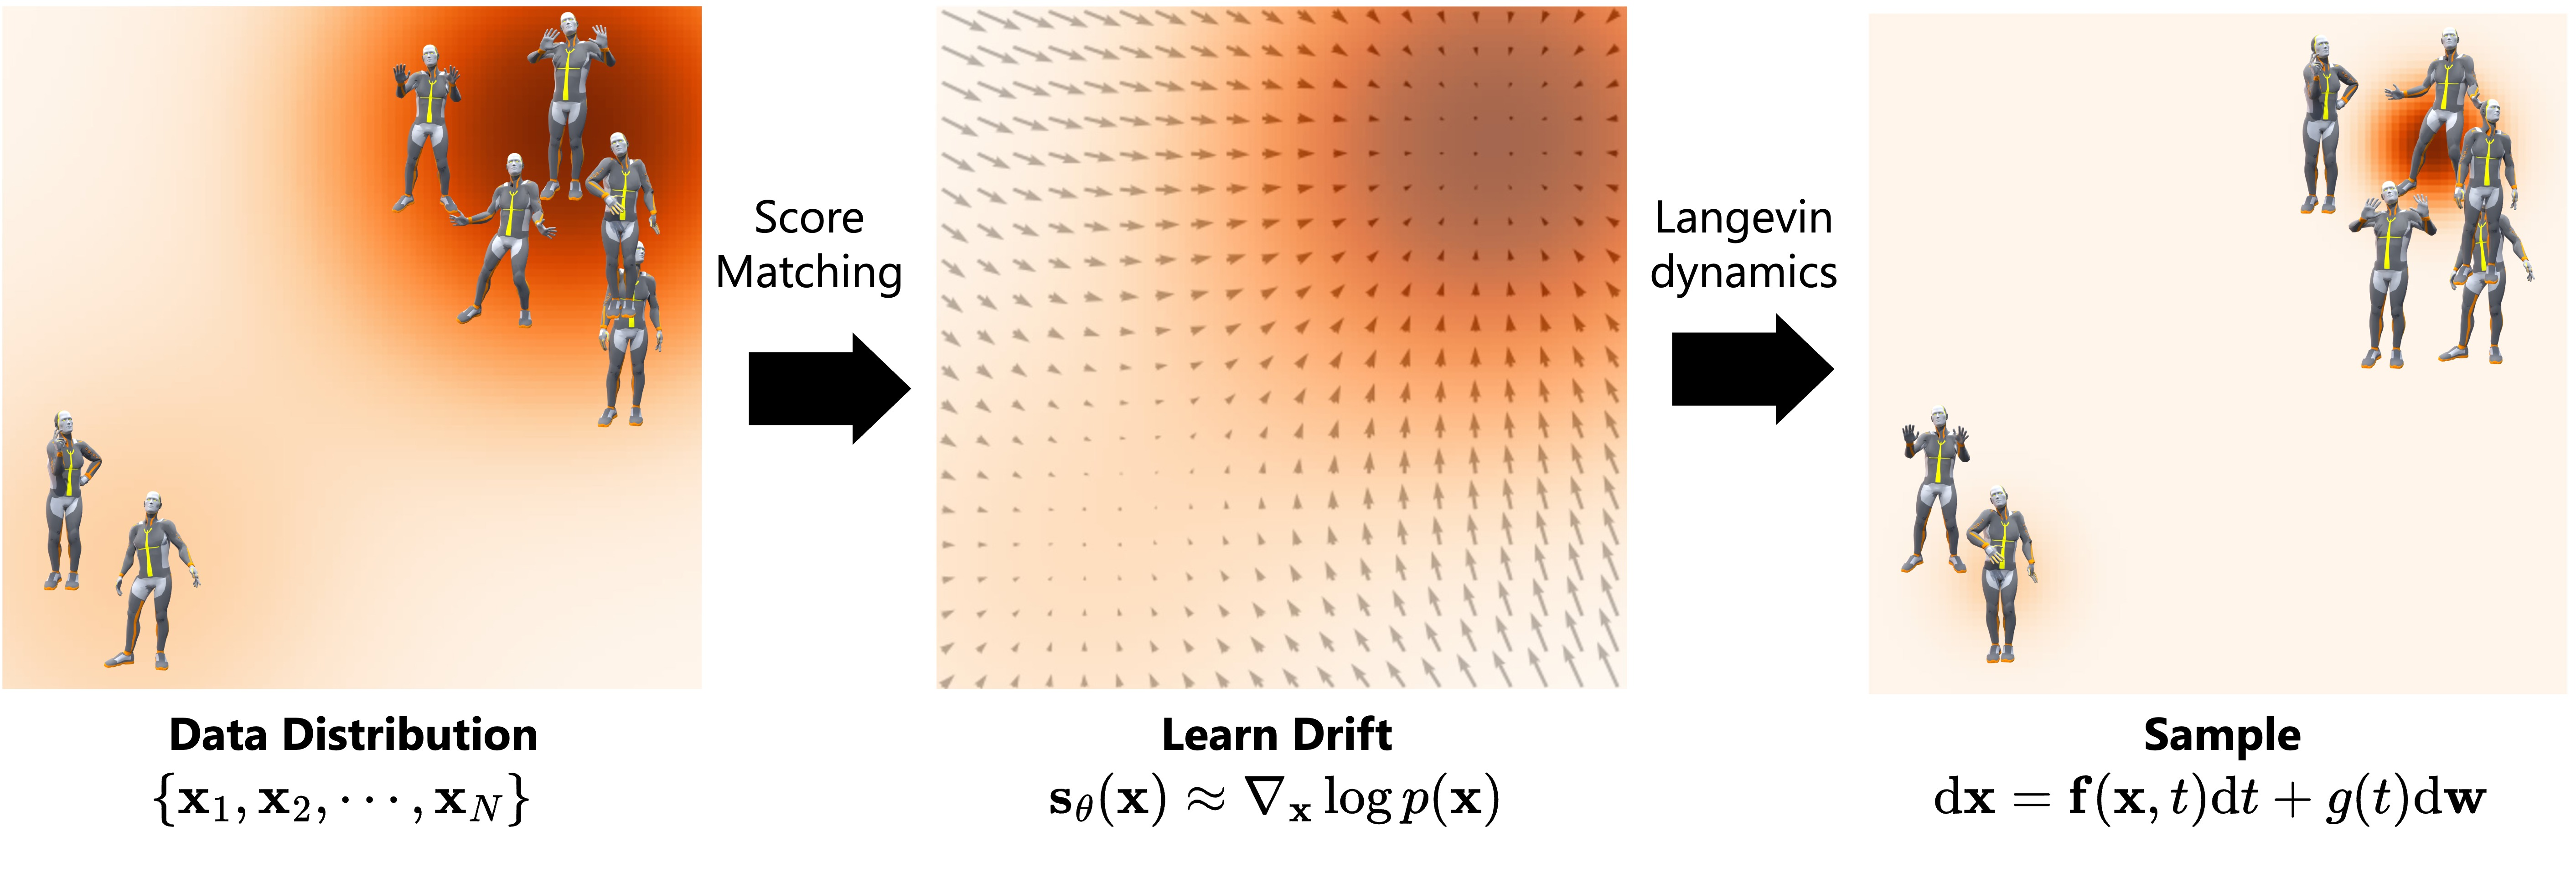
\includegraphics[width=\textwidth]{ScoreMatching}
	\caption{Minh hoạ nguyên lý chung của mô hình mô hình Diffusion.}
	\label{fig:ScoreMatching}
\end{figure}

Tương tự phương pháp trong nhóm phương pháp sinh ngầm định (Implicit Generative Models \autoref{sec:ImplicitGenerativeModels}), nguyên lý của mô hình Diffusion là học một hàm $f_{\theta}$ biểu diễn xu hướng (drift) của quá trình từ phân phối chuẩn $\mathcal{N}(0, \mathbf{I})$ về phân phối của dữ liệu $\bx_{0} \sim p(\bx)$, từ đó lấy mẫu (sampling) lên từng bước của quá trình đảo ngược để sinh ra các dữ liệu mới như \autoref{fig:ScoreMatching}.
Quá trình này được thực hiện từng $T$ bước, với nhiễu được thêm trong quá trình lấy mẫu giảm dần để mô hình có thể điều hướng về các vùng có mật độ dữ liệu lớn.

\subsection{Phương pháp tiêu biểu}
\label{subsec:TypicalMethod}

\subsubsection{Phương pháp tiêu biểu}

\begin{itemize}
	\item \textit{MotionDiffuse} \cite{zhang2022motiondiffuse} sử dụng mô hình Diffusion có điều kiện, với điều kiện dựa trên là văn bản mà không bao gồm âm thanh. Ngoài ra mô hình dự đoán nhiễu, chứ không dự đoán chuỗi cử chỉ gốc. Mô hình MotionDiffuse sử dụng các lớp Self-Attention và Cross Attention để tính tương quan giữa đặc trưng văn bản và đặc trưng cử chỉ trong công đoạn \textit{5. Kết hợp đặc trưng} (\autoref{fig:CommonStage}).
	
	\item \textit{Flame} \cite{kim2023flame} sử dụng mô hình diffusion với kiến trúc transformer. Trong công đoạn \textit{2. Xử lý đặc trưng} (\autoref{fig:CommonStage}), mô hình sử dụng mô hình pre-train RoBERTa để nhúng (embedding) văn bản để được các vector đặc trưng văn bản, và sử dụng chúng làm điều kiện cho mô hình. 
	Trong cộng đoạn \textit{5. Kết hợp đặc trưng} (\autoref{fig:CommonStage}), sử dụng văn bản làm token $\texttt{CLS}$ đầu tiên của chuỗi cử chỉ trước khi đi qua lớp Transformer Decoder .  Mô hình cũng dự đoán nhiễu đã được thêm vào mô hình Diffusion chứ không dự đoán chuỗi cử chỉ gốc.
	
	\item \textit{DiffWave} \cite{kong2020diffwave} sử dụng mô hình Diffusion với việc dự đoán nhiễu, các bước thời gian được đi qua nhiều lớp Fully Connected khác nhau và lớp kích hoạt Swish trước khi kết hợp các đặc trưng. Mô hình sử dụng kiến trúc dilated convolutions kế thừa từ WaveNet. Mô hình DiffWave giúp biểu diễn giọng nói được biểu diễn tốt hơn, tạo đầu vào hiệu quả hơn cho mô hình Diffusion.
	
	\item \textit{Listen, denoise, action} \cite{alexanderson2022listen} kế thừa từ mô hình DiffWave \cite{kong2020diffwave}, thay lớp dilated convolutions bằng Transformer , kết hợp với Conformers giúp cải thiện hiệu suất của mô hình.
	
	\item \textit{DiffSHEG} \cite{chen2024diffsheg} sử dụng mô hình diffusion, trong công đoạn \textit{2. Xử lý đặc trưng}, mô hình DiffSHEG sử dụng HuBERT để biểu diễn âm thanh. Coi biểu cảm là tín hiệu cho cử chỉ. Mô hình đạt được sự kết hợp thời gian thực của đồng thời cả biểu cảm khuôn mặt (facial expression) và cử chỉ (gesture).
	
	\item \textit{GestureDiffuCLIP} \cite{ao2023gesturediffuclip} sử dụng mô hình Diffusion với điều kiện là văn bản, GestureDiffuCLIP sử dụng phương pháp học tương phản (Contrastive Learning) để kết hợp đặc trưng văn bản thông qua CLIP để điều khiển phong cách của cử chỉ. Tương tự các phương pháp trên, coi văn bản như là Prompt của các mô hình sinh văn bản như StableDiffusion, Midjourney giúp mô hình học được cử chỉ từ đoạn văn bản mô tả.
	
	\item \textit{Freetalker} \cite{yang2024freetalker} sử dụng mô hình Diffusion để huấn luyện trên nhiều tập dữ liệu khác nhau, tạo cử chỉ cho người nói dựa trên lời nói và văn bản. Mô hình dự đoán cử chỉ gốc. Thay vì sử dụng Transformer, Freetalker sử dụng Attention-based Network để tính tương quan giữa các đặc trưng văn bản, âm thanh và cử chỉ trong công đoạn \textit{5. Kết hợp đặc trưng} (\autoref{fig:CommonStage}).
\end{itemize}


\subsubsection{Phương pháp được kết thừa trong luận văn}

\begin{itemize}
	\item \textit{MDM} \cite{tevet2022human}  áp dụng Diffusion có điều kiện cho bài toán sinh cử chỉ, với điều kiện là CLIP (Contrastive Language–Image Pre-training) của văn bản mô tả. MDM sử dụng kiến trúc transformer để tái tạo dữ liệu cử chỉ ban đầu, sử dụng Diffusion có điều kiện với điều kiện là đoạn văn bản mô tả chuyển động của cử chỉ. Tương tự các phương pháp diffusion sử dụng văn bản mô tả, trong công đoạn \textit{3. Trích xuất đặc trưng} (\autoref{fig:CommonStage}), đoạn văn bản sẽ được mặt nạ ngẫu nhiên (Random Mask) để ẩn đi các đoạn văn bản, từ đó giúp mô hình xác định mức độ quan trọng của từng đoạn văn bản đối với các cử chỉ khác nhau.
	%	Ở công đoạn 
	Trong công đoạn \textit{5. Kết hợp đặc trưng} (\autoref{fig:CommonStage}), mô hình sử dụng văn bản làm token $\texttt{CLS}$ đầu tiên của chuỗi cử chỉ trước khi đi qua lớp Transformer Encoder. Trong Transformer Encoder, cơ chế self-attention sẽ tính sự tương quan giữa văn bản với từng frame của cử chỉ. MDM dự đoán dữ liệu gốc thay vì dự đoán nhiễu.
	
	\item \textbf{DiffuseStyleGesture} \cite{yang2023diffusestylegesture} là mô hình Diffusion kế thừa từ \textit{MDM} \cite{tevet2022human}. Mô hình kết hợp điều kiện bao gồm âm thanh, cử chỉ khởi tạo và phong cách. Trong công đoạn \textit{1. Tiền xử lý} (\autoref{fig:CommonStage}) mô hình xử lý các tọa độ vector để thu được vectơ có số chiều $D=1141$ ở mỗi khung hình. Trong công đoạn \textit{2. Xử lý đặc trưng} (\autoref{fig:CommonStage}), DiffuseStyleGesture sử dụng WavLM để nhúng âm thanh. Trong công đoạn \textit{5. Kết hợp đặc trưng} (\autoref{fig:CommonStage}), mô hình cải tiến MDM bằng việc sử dụng Cross-Local Attention trước khi đi qua lớp Transformer Encoder.
%	 \textit{1. Tiền xử lý} (\autoref{fig:CommonStage}), dữ liệu cử chỉ $\bx^{J \times D}$ là số khung xương, với mỗi khung xương
\end{itemize}

\subsection{Mô hình Diffusion phù hợp với bài toán sinh cử chỉ}
\label{subsec:reason}

Với đặc điểm dữ liệu cử chỉ như giá trị của các góc quay và tọa độ điểm khớp, yêu cầu độ chi tiết cao đảm bảo độ chân thực cho chuyển động nhân vật. Tuy nhiên, dữ liệu trong các trường hợp cực trị của các tham số là rất hạn chế. Nhờ vào khả năng học chi tiết và bao quát dữ liệu trong các tình huống hiếm gặp. Mô hình Diffusion có thể giải quyết những khó khăn này, như được nêu trong \autoref{sec:difficult}. Mô hình Diffusion được đánh giá về ưu và nhược điểm so với các phương pháp hiện tại trong \autoref{table:CompareMethod}. Luận văn chọn mô hình Diffusion để giải quyết bài toán sinh cử chỉ. Mô hình của luận văn kế thừa từ mô hình \textbf{DiffuseStyleGesture} \cite{yang2023diffusestylegesture}, tích hợp văn bản như một đặc trưng ngữ nghĩa trong quá trình học trong công đoạn \textit{5. Kết hợp đặc trưng} (\autoref{fig:CommonStage}) của quá trình sinh cử chỉ để xây dựng mô hình đề xuất \textbf{OHGesture}.